\chapter{Experiments and simulations}\label{ch:experiments}

\section{Introduction}
This chapter describes the setups and procedures used for the experiments and MATLAB simulations in this thesis. A detailed description of the particle suspensions, microfluidic channels and chambers will be given here, such that the experiments can be repeated.

\section{Particle suspension}\label{sec:particleSuspension}
Commercially available superparamagnetic SiMAG-Silanol and ScreenMAG-Silanol beads of $1$ $\mu$m in size were obtained from Chemicell~\cite{chemicell2015}. Dynabeads MyOne, M270 and M280 were purchased from Thermo Fisher Scientific, UK. MyOne beads have a nominal diameter of $1.05$ $\mu$m, whereas M270 and M280 beads have a nominal diamter of $2.8$ $\mu$m~\cite{dynabeads2015}. Both manufacturers (Chemicell and Dynabeads) ship their beads already in suspension with an initial starting concentration as given in Table~\ref{tab:particleSuspensionMaterials}.

\begin{table}[htb]
\begin{center}
\caption[Bead types used in the experiments]{List of all bead types used in the experiments. The bead diameter and bead concentration listed is as given by the manufacturer.}
\vspace{1ex}
\label{tab:particleSuspensionMaterials}
\begin{tabular}{lclc}
\hline
Bead Type 	& Size 				& Supplier 	& Concentration\\ 
					& 	[$\mu$m]  	&  				& [beads/mL]\\
\hline
ScreenMAG-Silanol  	& $1.0 \pm 0.15$				& Chemicell GmbH 	& $9\times10^{10}$ \\
SiMAG-Silanol 			& $1.0 \pm 0.15$				& Chemicell GmbH  	& $9\times10^{10}$ \\
Dynabeads MyOne 	& $1.05 \pm 0.05$ 	& Thermo Fisher Scientific & $7-10\times 10^{9}$ \\
Dynabeads M280 		& $2.8 \pm 0.08$ 		& Thermo Fisher Scientific & $6-7\times10^{8}$ \\
Dynabeads M270 		& $2.8 \pm 0.08$ 		& Thermo Fisher Scientific & $6-7\times10^{8}$ \\  
\hline
\end{tabular}
\end{center}
\end{table}

Prior to the suspension preparation, the Dynabeads were washed three times following the protocol by Thermo Fischer. The washing solution used was phosphate buffered saline (PBS) with $0.01\%$ w/v BSA and $0.01\%$ v/v Tween-20. First, 1 mL of bead suspension was added to an equal volume of washing solution in an Eppendorf tube and vortexed for 5 seconds. Next, the Eppendorf tube was placed on a Neodyminum magnet ($25$ mm $\times$ $25$ mm $\times$ $5$ mm ) for at least 1 minute to pellet the beads. With the beads pelleted, the supernatant was removed. Next, the magnet was removed from the Eppendorf tube and the washed Dynabeads were re-suspended in deionized water. This procedure was repeated twice more.

To prepare the different bead suspensions, 1 mL of washed bead suspension was diluted either by $8$ mL, $7.5$ mL or $5.5$ mL of deionized (DI) water, depending on the initial bead concentration, to approximately produce whole number multiples of ten in concentration. From this concentrated bead suspension 1 mL was taken and diluted with 9 mL of DI water. This subsequent dilution step was performed multiple times in order to achieve concentrations which differ by one order of magnitude, ranging from $10^{5}$ to $10^{9}$ beads/mL. Between every dilution step, the suspension was vortexed for at least 30 seconds to make sure the beads were fully suspended and evenly dispersed. Note that the volume of the beads was assumed to be negligible in this dilution process. This is a valid assumption because the volume fraction of beads in the as-supplied bead suspension is in the order of $O(10^{-4})$. Finally, $0.1\%$ w/v of Pluronic F-127 and $0.01\%$ v/v of Tween-20 was added to prevent the beads from sticking together and adhering to the microfluidic channel surface. All the chemicals used to make the suspensions are listed in Table~\ref{tab:chemicalSuspensionMaterials} and are all commonly used in the literature for particle separation and sample preparation~\cite{Deng2002,Afshar2011,Rinklin2012,Samwer2013,Pamme2006a,Peyman2009,Tarn2013}.

\begin{table}[htb]
\begin{center}
\caption[Chemicals used in the experiments]{List of the chemicals used in the experiments to prepare the particle suspension.}
\vspace{1ex}
\label{tab:chemicalSuspensionMaterials}
\begin{tabular}{ll}
\hline
Chemical 	& Supplier\\ 
\hline
PBS 					& Life Technologies \\
Tween-20 		& Thermo Fisher Scientific\\
Pluronic F-127 	& Sigma-Aldrich \\
\hline
\end{tabular}
\end{center}
\end{table}

%\begin{table}[htb]
%\begin{center}
%\caption[Bead types and chemicals used in the experiments]{List of all bead types and chemicals used in the experiments.}
%\vspace{1ex}
%\label{tab:particleSuspensionMaterials}
%\begin{tabular}{lllll}
%\hline
%Type 	& Material 	& Supplier 	& Concentration\\ 
%			& 					&  				& [beads/mL]\\
%\hline
%\multirow{5}{*}{Beads} 	
% & ScreenMAG-Silanol 		& Chemicell GmbH & $1$ & $9\times10^{10}$ \\
% & SiMAG-Silanol 				& Chemicell GmbH & $1$ & $9\times10^{10}$ \\
% & Dynabeads MyOne 		& Thermo Fisher Scientific & $1.05 \pm 0.05$ & $7-10\times 10^{9}$ \\
% & Dynabeads M280 			& Thermo Fisher Scientific & $2.8 \pm 0.08$ & $6-7\times10^{8}$ \\
% & Dynabeads M270 			& Thermo Fisher Scientific & $2.8 \pm 0.08$ & $6-7\times10^{8}$ \\  
%\hline
%\multirow{3}{*}{Chemicals}  & PBS & Life Technologies \\
% & Tween-20 & Thermo Fisher Scientific\\
% & Pluronic F-127 & Sigma-Aldrich \\
%\hline
%\end{tabular}
%\end{center}
%\end{table}

\subsection{SEM imaging of magnetic beads}\label{subsec:semImaging}
To visualize the beads and to verify their size distribution, the particles were imaged using Scanning Electron Microscope (SEM) in the secondary electron mode. In this study an FEI\textsuperscript{\texttrademark} Quanta\textsuperscript{\texttrademark} 600 SEM was used; the accelerating voltage was set to $10$ kV to minimise charging effects during imaging. 

The samples for the SEM analysis were prepared as follows: $20$ $\mu$L of bead suspension with a concentration of $10^{6}$ beads/mL was pipetted on a $15$ cm silicon wafer, that had prior to the experiment been oxygen plasma treated to make its surface hydrophilic. The wafer was spun at $2000$ rpm for $30$ seconds, leaving a distribution of beads on the surface of the silicon wafer. Then, a $5$ nm thick gold layer was vapour deposited to enhance conductivity. 

\section{Microfluidic devices and chambers}\label{sec:microfluidicDevicesAndChambers}
Four different fluid devices are used throughout the work described in this thesis. The different devices are either channels, which allow a flow, or hydrostatic chambers. Each device will be described here and referenced back in the various chapters.

%Five different chip designs were employed for the work described in this thesis, though all featured common traits of a central separation/reaction chamber, as well as a particle inlet channel, multiple buffer/reagent channels and several outlet channels. Each of the designs will be described here and given a designation which will be referred to throughout the remainder of the thesis

\subsection{Microfluidic hydrodynamic focusing device}\label{subsec:microfluidicHydrodynamicFocusingChannel}
The device used for the hydrodynamic focusing was produced at Pusan National University in South Korea (PNU), using standard microfabrication techniques (soft lithography). The device comprised two fluid channels with three inlets and three outlets, as shown in Figure~\ref{fig:fluidChannelJuanSang}. These channels will be referred to as PNU 3in3 throughout this thesis. The main channel section has length of $35$ mm and width of $500$ $\mu$m. The three inputs have width of $200$ $\mu$m. By having three input channels, hydrodynamic focusing is possible, which allows for precise control of the middle inlet stream (sample stream). 

\begin{figure}[htb]
	\centering
   \includegraphics[width=0.7\textwidth]{img/chapters/chapter_3_experiment/fluidChannelJuanSang.png}
	\caption[Microfluidic hydrodynamic focusing device]{Schematic view of the microfluidic hydrodynamic focusing device, produced at Pusan National University using soft lithography. The design is symmetric with three inlets and outlets on either end. The three inlet channels allow for hydrodynamic focusing.}
\label{fig:fluidChannelJuanSang}
\end{figure}
%The device was produced using standard microfabrication techniques (soft lithography); see ~\cite{JeungSangGo2007} for further details. Briefly, a $50-100$ mm thick negative photoresist (SU-8 2050) is spin coated onto a substrate to form a cast. The photoresist is patterned by photolithography and hard baked. Ports for silicone tubes are added to the structure and covered with polydimethylsiloxane (PDMS). After the PDMS has hardened, it can be separated from the underneath structure and bonded onto a glass substrate.

\subsection{Microfluidic separation device}\label{subsec:microfluidicSeparationDevice}
In addition to the PNU 3in3 device another microfluidic device was obtained which was better suited for bead separation studies. A custom designed microfluidic channel was manufactured by iBidi GmbH in PDMS, to be more convenient for bead separation and hydrodynamic focusing of the injected beads. The design was based on a standard iBidi geometry of $\mu$-Slide III 3in1 modified to a $\mu$-Slide III 3in3 with three inlets and three outlets. The device has the following dimensions: length $24$ mm, width $3$ mm and depth $0.4$ mm. The three inlets and three outlets allow for hydrodynamic focusing at the inlet, and collection of the three separate fluid streams at the outlet. A schematic of the customized iBidi device is shown in Figure~\ref{fig:newMicrofluidChannelDesign}. 

\begin{figure}[htb]
        \centering
        \begin{subfigure}[b]{0.48\textwidth}
                \includegraphics[width=\textwidth]{img/chapters/chapter_3_experiment/customMicrofluidChannelDesign2D.png}
                \caption{}  
        \end{subfigure}
        \hfill
        \begin{subfigure}[b]{0.48\textwidth}
                \includegraphics[width=\textwidth]{img/chapters/chapter_3_experiment/customMicrofluidChannelDesign3D.png}
                \caption{}                
        \end{subfigure}
        \caption[Schematic of the customized iBidi $\mu$-slide]{A schematic of the customized iBidi $\mu$-slide, with a length of $24$ mm, a width of $3$ mm and a depth of $0.4$ mm. (a) Top view of the microfluidic separation device. (b) 3D model of the iBidi $\mu$-Slide III 3in3.}
        \label{fig:newMicrofluidChannelDesign}
\end{figure}
%\begin{figure}[htb]
%   \centering
%   \includegraphics[width=0.55\textwidth]{img/chapters/fluidMechanics/customMicrofluidChannelDesign2.png}
%   \caption[Schematic of the customized iBidi $\mu$-slide]{A schematic of the customized iBidi $\mu$-slide, with a length of $24$ mm, a width of $3$ mm and a depths of $0.4$ mm.}
%   \label{fig:newMicrofluidChannelDesign}
%\end{figure}

\subsection{Microfluidic counting slide}\label{subsec:microfluidicCountingSlide}
To observe beads, a FastRead 102 microscope counting slide (Immune Systems, UK) was used. The FastRead 102 is a disposable plastic device composed of a set of $10$ easy-to-fill fluid \textit{observation chambers}, as depicted in Figure~\ref{fig:fastRead102}. Each observation chamber has a depth of 100 $\mu$m and a counting grid etched into its surface, as illustrated in the magnification section of Figure~\ref{fig:fastRead102}. The counting grid has a dimension of $5$ mm $\times$ $2$ mm and is divided into $10$ squares. Each square is further divided into $16$ smaller squares.

\begin{figure}[htb]
	\centering
   \includegraphics[width=0.7\textwidth]{img/chapters/chapter_3_experiment/fastRead.eps}
	\caption[FastRead 102 Slide schematic]{Schematic illustration of a FastRead 102. The magnifying glass shows a close up view of a single observation chamber.}
\label{fig:fastRead102}
\end{figure}

\subsection{Hydrostatic fluid chamber}\label{subsec:hydrostaticFluidChamber}
It is convenient to use a single observation chamber for easy access by the permanent magnet. Either a FastRead 102 slide can be cut down or a simple hydrostatic fluid chamber can be constructed from simple components. The hydrostatic fluid chamber shown in Figure~\ref{fig:hydrostaticFluidChamber} was assembled from standard glass microscope slides and No. $1.5$ glass cover slips, purchased from Agar Scientific Ltd. To create the chamber, two thin strips of cover slip are first cut using a diamond-tipped scribe and then bonded to the face of the bottom microscope slide using varnish (Rimmel London, 60 seconds). The top microscope slide is then bonded before leaving the device to cure for a minimum of two hours. Once the device is cured, the aqueous suspension of magnetic beads is drawn into the channel via capillary action and then sealed around all edges with varnish to ensure that it is water-tight.

\begin{figure}[htb]
	\centering
   \includegraphics[width=0.75\textwidth]{img/chapters/chapter_3_experiment/cuvette.pdf}
	\caption[Hydrostatic fluid chamber fabrication procedure]{Fabrication procedure of the hydrostatic fluid chamber. (1) Glass microscope slides are cut in squares. (2) Standard glass cover slips are cut in thin strips and glued to the bottom microscope slide using varnish. (3) Another cut microscope slide is bonded to the top of the structure. (4) After the chamber is filled with a particle suspension, the chamber is sealed around all edges and openings with varnish.}
\label{fig:hydrostaticFluidChamber}
\end{figure}

These single chambers can be rapidly and reproducibly made and use minimal amounts of the suspension, making them suitable for use in the equilibrium position experiments (see Section~\ref{sec:equilibriumPositionExperiment}). The only drawback, compared to the FastRead 102 slides, is that there is no patterned grid for counting or locating beads.

\section{Magnetic field measurement}\label{sec:magneticForceMeasurement}
The magnetic flux density of a N42 neodymium bar magnet with dimensions $42$ mm $\times$ $8$ mm $\times$ $10$ mm (Magnets4U, UK) was measured using a hand-held Hall sensor (5170 Gauss/Tesla Meter, F.W. Bell). The Hall probe is constructed from a thin sheet of semiconductor with output connections perpendicular to the direction of current flow. When subjected to a magnetic field, the Hall probe responds with an output voltage proportional to the magnetic flux density.

The flux density of the bar magnet was measured by moving the transversal Hall probe away from the magnet along its centreline to $48$ mm from its surface. The Hall probe was mounted on a precision translational moving stage and was manually  moved in step sizes of $0.1$ mm. The Hall probe was maintained perpendicular to the flux lines in order to maximise the output signal. 

The Double Magnet configuration was measured in the same way. For the Double Magnet configuration two rectangular N42 Neodymium magnets ($20$ mm $\times$ $6$ mm $\times$ $1.5$ mm) were arranged on top of each other, leaving an air gap of $2$ mm in between. The Hall probe was kept in the centre plane between the two magnets. The probe was moved from the centre point between the two magnets up to $17$ mm away from the outer edge of the two magnets with a step size of $0.5$ mm.

Prior to each measurement, the Hall sensor was re-calibrated inside a zero flux chamber. Photographs of both measurement setups, for the single bar magnet as well as the Double Magnet configuration, are presented in Figure~\ref{fig:magneticFluxDensityMeasurementExperiment}.

\begin{figure}[htb]
        \centering
        \begin{subfigure}[t]{0.48\textwidth}
                \includegraphics[width=\textwidth]{img/chapters/chapter_3_experiment/magneticForceMeasurementSetup_white_withScaleBar.pdf}
                \caption{Single bar magnet setup measurement}
        \end{subfigure}
        \hfill
        \begin{subfigure}[t]{0.48\textwidth}
                \includegraphics[width=\textwidth]{img/chapters/chapter_3_experiment/magneticForceMeasurementSetupDoubleMagnet_white_withScaleBar.pdf}
                \caption{Double Magnet configuration measurement}
        \end{subfigure}  
        \caption[Magnetic flux density measurement setup]{Setup to measure the magnetic flux density of different magnet configurations: (a) single bar magnet. (b) double magnet configuration.}
        \label{fig:magneticFluxDensityMeasurementExperiment}
\end{figure}

\section{Magnetophoretic mobility experiment}\label{sec:magnetophoreticMobilityExperiment}
To compare the mobility of individual magnetic microparticles, a cell tracking velocimetry (CTV) setup was assembled to enable measurements of the magnetophoretic velocity of single beads in stationary liquid (DI water) within a region of known magnetic field. The magnetic beads were optically observed in a FastRead 102 microscope counting slide (see Section~\ref{subsec:microfluidicCountingSlide}). The rectangular grid structure, which is etched onto each observation chamber, allows determination of the exact view location within the chamber and thus the precise distance between the magnet and the currently observed bead. The magnetic beads moving towards the magnet were video recorded using an inverted microscope (Leitz Wetzlar, Germany) with a long working distance $20\times$ objective lens (Comar Optics, Cambridge, UK) and a CCD camera ($\mu$Eye Imaging Development Software, Germany). The resolution of the inverted microscope  system allowed the clear viewing of individual beads of $1$ $\mu$m to $2.8$ $\mu$m in diameter. The recorded trajectories of individual beads moving towards the magnet were analysed off-line using the freely available software \textit{ImageJ}. The magnetically induced velocity was calculated using the open source particle tracking plug-in \textit{MTrackJ}.

Prior to the measurement, the beads had been diluted to a suspension of $0.9-1.4\times 10^{5}$ beads/mL as described in Section~\ref{sec:particleSuspension}. The concentrations were confirmed by observing the density of beads on the counting grid of the observation chamber. Visual inspection of previous experiments had shown that such low concentrations successfully avoid bead interaction~\cite{Oduwole2016}. Before each experiment, bead suspensions were sonicated in an ultrasonic bath for at least five minutes to break up aggregates and fully suspend the beads. A volume of $20$ $\mu$L of the sonicated suspension was pipetted into an observation chamber assisted via capillary action. Once the beads had become stationary, an external magnetic field was applied by accurately positioning an N42 neodymium (NdFeB) magnet ($42$ mm $\times$ $8$ mm $\times$ $10$ mm) adjacent to the FastRead 102 counting slide. The FastRead 102 counting slide was cut down in size in order to be placed at a minimum distance of $10$ mm from the magnet. When the magnet is moved $40$ mm away from the chamber's edge the motion of the beads was observed to be negligible and was thus used as the 	magnet \textit{parking} position. The permanent magnet was attached to a high precision translation stage, which allowed accurate movement of the magnet to different positions from the counting grid, while keeping the view location within the chamber stationary. This configuration enabled the magnetic field experienced by the beads to be accurately adjusted. A photograph of the CTV setup is shown in Figure~\ref{fig:magnetophoreticMobilityExperiment}.

\begin{figure}[htb]
	\centering
   \includegraphics[width=0.6\textwidth]{img/chapters/chapter_3_experiment/magnetophoreticMobilityMeasurementExperiment.pdf}
	\caption[Magnetophoretic velocity measurement experiment setup]{Setup to measure the magnetically induced velocity. The magnet ($42$ mm $\times$ $10$ mm $\times$ $8$ mm) is mounted on a high precision translation stage to move the magnet with respect to the observation chambers.}
\label{fig:magnetophoreticMobilityExperiment}
\end{figure}

\section{SQUID measurement}\label{sec:squidMeasurement}
For the purpose of simulating the bead trajectories accurately, it is necessary to know their magnetic susceptibility. The susceptibility of magnetic beads was independently measured using a SQUID measurement system (Quantum Design Magnetic Property Measurement System MPMS-XL). A sample ($1-30$ mg) of the different magnetic bead types listed in Table~\ref{tab:particleSuspensionMaterials} was dried in an oven at $65^\circ$ C. The dry beads were placed in a sample capsule. The sample capsule was put in a \textit{straw} (sample holder) and both ends were filled with empty capsules in order to keep the sample capsule at an appropriate height within the holder. The sample holder was  sealed and attached to the SQUID probe. The probe is lowered into the SQUID measurement system where a magnetic field up to $\pm5$ Tesla is applied at a stabilised temperature of $300$ K. The different sample preparation steps are depicted in Figure~\ref{fig:squidSamplePerparation}. The results of the SQUID measurements and discussion are in Section~\ref{sec:magnetizationOfSuperparamagneticParticles}.

\begin{figure}[htb]
	\centering
   \includegraphics[width=0.6\textwidth]{img/chapters/chapter_3_experiment/squidMeasurement.pdf}
	\caption[SQUID experiment sample holder preparation]{Different steps to prepare the SQUID sample. (1)-(2) The dried particles are placed in an empty capsule, which will be the sample capsule. (3) The sample capsule is then put in a \textit{straw} (sample holder). To have the sample capsule at a fixed height within the straw, both ends are filled with empty capsules and sealed with tape. The straw is attached to a SQUID probe and then lowered into the SQUID measurement system. Figure is not drawn to scale.}
\label{fig:squidSamplePerparation}
\end{figure}

\section{Hydrodynamic focusing}\label{sec:hydrodynamicFocusing}
The hydrodynamic focusing was numerically simulated and experimentally verified. A detailed description of the numerical and experimental setup is given here.  
 
\subsection{Hydrodynamic focusing simulation}\label{subsec:hydrodynamicFocusingSimulation}
In order to simulate the fluid dynamics in the microfluidic channel, a three dimensional (3D) symmetric geometry, representing the entrance of the iBidi $\mu$-slide microfluidic channel (see Section~\ref{subsec:microfluidicSeparationDevice}), including the three inlets, was modelled in ANSYS Design Modeller (see Figure~\ref{fig:hydrodynamicFocusingSimulation}). The model was meshed by a fine hexahedral mesh with $464,558$ elements and $91,424$ nodes. Increasing the number of points beyond this was found to have no noticeable impact on the output of the model (i.e. grid independence). Figure~\ref{fig:hydrodynamicFocusingSimulationMesh} shows the top half of the meshed model. Only the top half of the channel is computed due to symmetry, which is equivalent to a symmetry boundary condition at $y=0$.

\begin{figure}[htb]
        \centering
        \begin{subfigure}[b]{0.35\textwidth}
                \includegraphics[width=\textwidth]{img/chapters/chapter_3_experiment/fluidChannelEntrance.pdf}
                \caption{}
                \label{fig:hydrodynamicFocusingSimulation}  
        \end{subfigure}
        \hfill
        \begin{subfigure}[b]{0.55\textwidth}
                \includegraphics[width=\textwidth]{img/chapters/chapter_3_experiment/hydrodynamicFocusingSimulationMesh.png}
                \caption{}    
                \label{fig:hydrodynamicFocusingSimulationMesh}            
        \end{subfigure}
        \caption[3D model of entrance of the microfluidic iBidi channel]{3D model of the entrance of the microfluidic iBidi channel used for the simulation of the hydrodynamic focusing. (a) Modelled entrance of the channel including the three inlet channels. The arrows indicate the simulated direction of flow. (b) 3D mesh model used for the finite element method simulations of the hydrodynamic focusing effect. The model was hexahedral meshed with $464,558$ elements and $91,424$ nodes. The model represents only the upper half of the entrance ($y>0$), with the bottom half simulated using a symmetry condition.}
\end{figure}

All liquids were modelled as water at room temperature with \textit{no-slip} boundary conditions applied to all side-walls. Thus, all walls were set to no flux and the diffusion constant to $2.2\times10^{-11}$ m$^{2}$/s (self-diffusion of water). Only the continuous liquid phase was modelled and the effect of the suspended particles was neglected due to their size and low concentration ($\upsilon_{p} < 10^{-6}$). This allowed solutions of the flow in the microfluidic channel in an uncoupled manner (see Section~\ref{subsec:particleLadenFlowInMicrofluidicSystems}), i.e. only the fluid phase was simulated using an Eulerian approach. The three inlets were treated as laminar inflows with a set flow rate. The outlet is pressure controlled and set to atmospheric pressure. The model equations were solved by finding a steady solution for the velocity field of all flows.

\subsection{Hydrodynamic focusing experiment}\label{subsec:hydrodynamicFocusingExperiment}
The hydrodynamic focusing experiments were performed to test the viability to accurately focus the inlet sample stream in two different fluid channel designs; PNU 3in3 and iBidi $\mu$-Slide III 3in3. Both designs are described in Section~\ref{subsec:microfluidicHydrodynamicFocusingChannel} and Section~\ref{subsec:microfluidicSeparationDevice} and used in the study described below. 

The three inlets were connected to three $1.0$ mL glass syringes (BD Biosciences, UK) using $0.5$ mm inner diameter flexible hard plastic (PTFE) tubing (Microfluidic ChipShop) to introduce the flows to the device. Silicone tubes with an inner diameter of $0.76$ mm (Microfluidic ChipShop) were used as a sleeve to connect the hard plastic tubes with the syringe and microfluidic device via its respective interface. The interface of the two devices either requires an intermediate tube or a Male Luer fluid connector (Microfluidic ChipShop). Figure~\ref{fig:interfaceTubingConnection} shows the interface and tubing connections of the iBidi $\mu$-Slide III 3in3. Syringes were mounted on Harvard Apparatus syringe pumps (Harvard Apparatus, Standard Infuse/Withdraw Syringe Pump 11 Plus). 

\begin{figure}[htb]
	\centering
	\begin{subfigure}[b]{0.48\textwidth}
		\includegraphics[width=\textwidth]{img/chapters/chapter_3_experiment/deviceInterfaces_labelled.pdf}
         \caption{}
		\label{fig:interfaceTubingConnection}  
    \end{subfigure}
    \hfill
	\begin{subfigure}[b]{0.48\textwidth}
		\includegraphics[width=\textwidth]{img/chapters/chapter_3_experiment/hydrodynamicFocusingExperimentSetup.pdf}
         \caption{}    
		\label{fig:hydrodynamicFocusingExperimentSetup}            
	\end{subfigure}
	\caption[Tubing connections to iBidi $\mu$-Slides III 3in3 interface for the hydrodynamic focusing experiment]{(a) Connections and tubing for the $\mu$-Slides III 3in3. Flexible hard plastic tubes were used to introduce the fluid to the device.  Silicone sleeves were mounted on a Male Luer fluid connector to interconnect the hard plastic tubes. (b) Setup of the hydrodynamic focusing experiment. Fluid is introduced through the three inlets and leaves the device through the three outlets. The ends of the outlet tubes were submerged in a single collection pot to avoid siphoning effects at low flow rates.}
\end{figure}

The outlet channels were either connected by tubing to a single external collection pot or directly connected to separate $500$ $\mu$L collection tanks (Microfluidic ChipShop) mounted on the iBidi $\mu$-Slide III 3in3 device. In the case where tubing was used, to avoid siphoning effects care was taken to keep the ends of the tubes below height of the microfluidic device while having the tubing ends submerged in water at all times, as shown in Figure~\ref{fig:hydrodynamicFocusingExperimentSetup}.

The three syringe pumps allowed independent control of the sheath and sample sample flow rate. In order to make the focusing effect visible, DI water was used as the sheath flow and ink (Pelikan, Royal Blue 4001) diluted in water was used as the inlet sample stream. The DI water was filtered prior to the experiment using a Millipore syringe filter (Whatman GE Healthcare) with a pore size of $1.0$ $\mu$m to reduce the risk of blocking the channels during the experiment.

Prior to any experiments it was necessary to coat the inside walls of the microfluidic device with a surfactant. This step was absolutely crucial to reduce the risk of air bubbles getting stuck in the device. A $10\%$ w/v ratio (with water), of Sigma-Aldrich F-127 non-ionic surfactant was used for this purpose (Sigma-Aldrich). This solution was flushed through the device before each experiment for $10$ minutes at a flow rate of $1$ mL/min. The microfluidic device was then filled with DI water, assuring no air bubbles were trapped. Trapped air bubbles could be conveniently flushed using higher flow rates. 

Before images of the hydrodynamic focusing effect were taken, the experiment was run for at least $30$ seconds, in order to establish steady state. Images were taken with a CCD camera ($\mu$Eye Imaging Development Software, Germany) mounted on a stereo microscope (Optika SZM-1 LED stereo microscope) with a $4\times$ magnification. 

\section{Magnet configurations}\label{sec:magneticSeparationConfigurations}
Two magnet configurations, Double Magnet  and Quadrupole, have been used for magnetic bead enrichment. All configurations used N42 Neodymium (NdFeB) magnets (First4Magnets$^\textsuperscript{\textregistered}$,UK) with a dimension of $20$ mm $\times$ $6$ mm $\times$ $1.5$ mm. 

\subsection{Double Magnetic configuration}\label{subsec:doubleMagneticConfiguration}
The Double Magnet configuration shown in Figure~\ref{fig:doubleMagnetConfigurationExperiment} consisted of two NdFeB magnets. Both magnets were placed on the same side of the microfluidic separation device such that the edge of the magnets was $1.65$ mm away from the microfluidic channel edge. The two magnets were arranged in an attractive configuration, with both magnetizations pointing in the same direction, while having the microfluidic separation device clamped in between. The vertical separation between the two magnets was adjusted to be $2.6$ mm. In order to have a $2.6$ mm vertical separation and thus have the centre of the fluid channel along the $y$ direction, a microscope slide was inserted as a spacer between the iBidi $\mu$-Slide and the bottom magnet. The two magnets were conveniently aligned by eye, being held in place by the attractive magnetic force. The magnets and the spacer were robustly held in position with respect to the microfluidic channel, as shown in Figure~\ref{fig:doubleSide}.

\begin{figure}[htb]
\centering
	\begin{subfigure}[b]{0.48\textwidth}
		\includegraphics[width=\textwidth]{img/chapters/chapter_3_experiment/doubleMagnetConfigurationExperiment.pdf}
		\caption{Top view}
		\label{fig:doubleTop}
    \end{subfigure}
	\hfill
	\begin{subfigure}[b]{0.48\textwidth}
		\includegraphics[width=\textwidth]{img/chapters/chapter_3_experiment/doubleMagnetConfigurationSideExperiment.pdf}
		\caption{Side view}
		\label{fig:doubleSide}
	\end{subfigure}
	\begin{subfigure}[b]{0.8\textwidth}
	\centering
	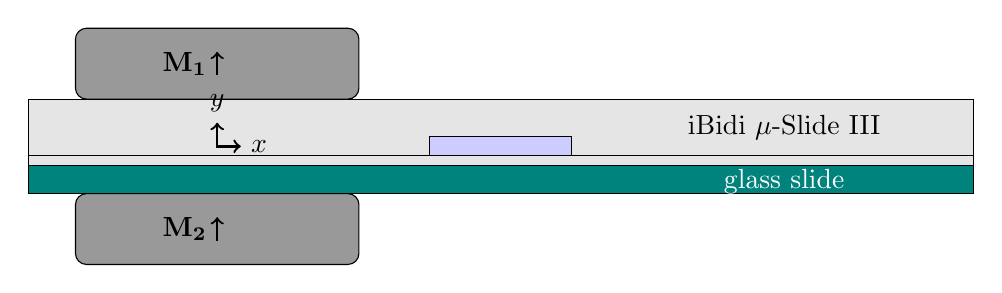
\begin{tikzpicture}[scale=0.6]
	\filldraw[rounded corners, fill=black!40!white, draw=black] (-9,1) rectangle (-3,2.5);
	\filldraw[rounded corners, fill=black!40!white, draw=black] (-9,-1) rectangle (-3,-2.5);	
	\draw[thick,->] (-6,1.5) -- node[thick,anchor=east]{$\mathbf{M_{1}}$} (-6,2.0);
	\draw[thick,->] (-6,-2.0) -- node[thick,anchor=east]{$\mathbf{M_{2}}$} (-6,-1.5);

	\filldraw[fill=black!10!white, draw=black] (-10,-0.2) rectangle (10,1);
	\filldraw[fill=black!10!white, draw=black] (-10,-0.4) rectangle (10,-0.2);
	\filldraw[fill=green!51!blue, draw=black] (-10,-1) rectangle (10,-0.4);	
	\filldraw[fill=blue!20!white, draw=black] (-1.5,-0.2) rectangle (1.5,0.2);			
	
	\node[thick] at (6,0.4) {iBidi $\mu$-Slide III};	
	\node[thick,white] at (6,-0.75) {glass slide};	
		
	\draw[line width=0.3mm,<->] (-6,0.5) node[anchor=south] {$y$} -- (-6,0) -- (-5.5,0)node[anchor=west] {$x$};
	\end{tikzpicture}	
	
	\caption{Cross section schematic}
	\label{fig:doubleCrossSection}
	\end{subfigure}
\caption[Experimental setup of the Double Magnet configuration]{Experimental setup of the Double Magnet configuration. Two permanent magnets ($20$ mm $\times$ $6$ mm $\times$ $1.5$ mm) were located adjacent to the 3in3 fluid channel with the iBidi $\mu$-Slide III 3in3 held in between. (a) Top view of the Double Magnet configuration. (b) Side view of the Double Magnet configuration (c) 2D slice diagram ($z=0$) of the Double Magnet configuration. The permanent magnets (grey) were configured in attraction, with their magnetization vectors $\mathbf{M}$ pointing in the same direction. The microfluidic channel (light blue) was located to the right of the dipole configuration and was centred along $y$ by using a microscope glass slide (turquoise) as a spacer.}
\label{fig:doubleMagnetConfigurationExperiment}
\end{figure}

\subsection{Quadrupole configuration}\label{subsec:quadrupoleMagneticConfiguration}
The Quadrupole configuration shown in Figure~\ref{fig:quadrupoleMagnetConfigurationExperiment} featured four NdFeB magnets, basically two Double Magnet configurations on either side of the 3in3 fluid channel. Each Double Magnet had its magnetization in the same direction (i.e. in attraction), but the two Double Magnets were configured repelling each other. In order to overcome the repelling force and to have a horizontal separation of $3.5$ mm, an acrylic glass frame was made to keep the magnets in place (not shown in Figure~\ref{fig:quadrupoleMagnetConfigurationExperiment}).

As for the Double Magnet configuration described above (see Section~\ref{subsec:doubleMagneticConfiguration}), a microscope glass slide was inserted between the iBidi $\mu$-Slide III 3in3 and the two bottom magnets in order to keep the 3in3 microfluid channel centred along the $y$ direction, as shown in Figure~\ref{fig:quadrupoleSide}.

\begin{figure}[htb]
\centering
	\begin{subfigure}[b]{0.48\textwidth}
		\includegraphics[width=\textwidth]{img/chapters/chapter_3_experiment/quarupoleMagnetConfigurationExperiment.pdf}
		\caption{Top view}
		\label{fig:quadrupoleTop}
    \end{subfigure}
	\hfill
	\begin{subfigure}[b]{0.48\textwidth}
		\includegraphics[width=\textwidth]{img/chapters/chapter_3_experiment/quarupoleMagnetConfigurationSideExperiment.pdf}
		\caption{Side view}
		\label{fig:quadrupoleSide}
	\end{subfigure}
	\begin{subfigure}[b]{0.8\textwidth}
	\centering
	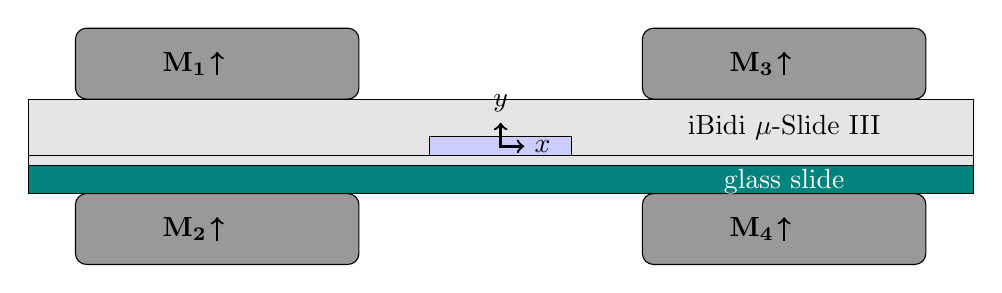
\begin{tikzpicture}[scale=0.6]
	\filldraw[rounded corners, fill=black!40!white, draw=black] (-9,1) rectangle (-3,2.5);
	\filldraw[rounded corners, fill=black!40!white, draw=black] (-9,-1) rectangle (-3,-2.5);	
	\draw[thick,->] (-6,1.5) -- node[thick,anchor=east]{$\mathbf{M_{1}}$} (-6,2.0);
	\draw[thick,->] (-6,-2.0) -- node[thick,anchor=east]{$\mathbf{M_{2}}$} (-6,-1.5);

	\filldraw[fill=black!10!white, draw=black] (-10,-0.2) rectangle (10,1);	
	\filldraw[fill=black!10!white, draw=black] (-10,-0.4) rectangle (10,-0.2);	
	\filldraw[fill=green!51!blue, draw=black] (-10,-1) rectangle (10,-0.4);	
	\filldraw[fill=blue!20!white, draw=black] (-1.5,-0.2) rectangle (1.5,0.2);					
	\filldraw[rounded corners, fill=black!40!white, draw=black] (9,1) rectangle (3,2.5);
	\filldraw[rounded corners, fill=black!40!white, draw=black] (9,-1) rectangle (3,-2.5);	
	\draw[thick,->] (6,1.5) -- node[thick,anchor=east]{$\mathbf{M_{3}}$} (6,2.0);
	\draw[thick,->] (6,-2.0) -- node[thick,anchor=east]{$\mathbf{M_{4}}$} (6,-1.5);
	
	\node[thick] at (6,0.4) {iBidi $\mu$-Slide III};	
	\node[thick,white] at (6,-0.75) {glass slide};	

	\draw[line width=0.3mm,<->] (0,0.5) node[anchor=south] {$y$} -- (0,0) -- (0.5,0)
	 node[anchor=west] {$x$};
	\end{tikzpicture}	
	\caption{Cross section schematic}
	\label{fig:quadrupoleCrossSection}
	\end{subfigure}
\caption[Experimental setup of the Quadrupole configuration]{Experimental setup of the Quadrupole configuration. Four permanent magnets ($20$ mm $\times$ $6$ mm $\times$ $1.5$ mm) were located next to the 3in3 fluid channel with two magnets on either side of the 3in3 fluid channel and with the iBidi $\mu$-Slide III 3in3 clamped in between. (a) Top view, (b),  side view and (c) 2D slice diagram ($z=0$) of the Quadrupole configuration. The permanent magnets, iBidi $\mu$-Slide III 3in3  and spacer, to keep the channel centred in $y$ direction, are indicated by different colours; i.e. grey, light blue and turquoise, respectively.}
\label{fig:quadrupoleMagnetConfigurationExperiment}
\end{figure}

\section{Static gathering points experiments}\label{sec:equilibriumPositionExperiment}
To verify the magnetic field pattern of the Double Magnet configuration and the existence of the static gathering point beyond the magnets, a specially made setup was built, as shown in Figure~\ref{fig:staticGatheringPointExperiment}. The setup had several degrees of freedom for flexibility, allowing the magnet height (Section~\ref{subsec:magnetHeightVariation}) and the vertical separation between the two magnets (Section~\ref{subsec:magnetVerticalSeparationVariation}) to be varied.

\begin{figure}[htb]
	\centering
	\includegraphics[width=0.9\textwidth]{img/chapters/chapter_3_experiment/staticGatheringLineExperimentalSetupOneFigure.pdf}
	\caption[Experimental setup to verify static gathering points]{Experimental setup to verify the static gathering points of the Double Magnet configuration. Magnets and microfluidic chamber are mounted onto L-brackets which can be accurately adjusted using precision lateral translation stages. The degrees of freedom of the setup are shown in the close up schematic. The schematic is not drawn to scale.}
\label{fig:staticGatheringPointExperiment}
\end{figure}

In these experiments, two N42 NdFeB magnets (First4Magnets$^\textsuperscript{\textregistered}$,UK) with a length, width and height of $20$ mm, $6$ mm and $1.5$ mm, respectively, were mounted onto aluminium holding blocks using Araldite$^\text{\textregistered}$ adhesive. The holding blocks were screwed onto L-brackets and could be removed to change the magnets. The L-brackets were mounted onto precision linear translation stages for accurate control of the vertical gap and height of the Double Magnet configuration, as shown in Figure~\ref{fig:staticGatheringPointExperiment}. Nonmagnetic materials were used to minimise the distortion of the magnetic field; the holding blocks and L-brackets were fabricated from aluminium and the fasteners were brass. The holding blocks and L-brackets were manufactured by the Oxford University workshop based on schematics drawn by the author. The schematic diagram in Figure~\ref{fig:staticGatheringPointExperiment} shows the Double Magnet configuration and illustrates the direction of movement of the magnets as well as the location of the fluid chamber. 

In all experiments, a hydrostatic chamber was chosen to visualize the beads' static gathering positions, because these experiments did not require continuous sample flows. The hydrostatic chambers were prepared according to Section~\ref{subsec:hydrostaticFluidChamber} and then filled with bead suspensions before being mounted onto the L-bracket. Suspensions of all considered bead types (see Table~\ref{tab:particleSuspensionMaterials}) were used in the experiments, where the concentration was varied between $\approx10^6$ beads/mL to $\approx10^8$ beads/mL ($\upsilon_{p} \approx {10^-8}-{10^-4}$). These high concentrations were chosen, in order to make the gathering positions clearly visible. 

Initially, the L-bracket, with the hydrostatic cover slip chamber, was positioned away from the magnets so that the beads within the chamber did not have any significant interaction with the field. The cover slip chamber was then slowly moved towards the magnets using the horizontal positioning stage. Moving the chamber slowly caused the beads to be repelled away from the magnets towards the position of static equilibrium, therefore increasing the concentration along the equilibrium line. When the chamber was correctly placed, the setup was left for two minutes to ensure the beads have reached their static gathering point and no further observable growth in particle agglomeration could be seen. A microscope (Optika SZM-1 LED stereo microscope) with a lower magnification (maximum magnification of $4\times$) gave a better visualisation of the overall structure of the formed band.

Pictures were taken with the CCD camera attached to the microscope and the gathering position was measured as being the distance from the centre axis of the equilibrium band to the edge of the magnets. The experiment could be repeated with the same chamber after $5$ minutes of sonication to break up agglomerations.

\subsection{Magnet height variation}\label{subsec:magnetHeightVariation}
In order to increase the height of the magnet, multiple N42 neodymium magnets with dimensions $20$ mm $\times$ $6$ mm $\times$ $1.5$ mm were stacked on top of each other on both sides of the L-brackets. In this manner, the assembled magnets can increment in height between $1.5$ mm and $6.0$ mm. 

The vertical separation between the two magnet stacks was kept at $2$ mm and only the height of each magnet stack was varied. In order to ensure the $2$ mm gap, microscope cover slips were used as spacers because the attractive force between the two magnet stacks was sufficient to close the gap without spacers, which would make the separation distance uncertain when the attractive force was significant.

\subsection{Magnet vertical separation variation}\label{subsec:magnetVerticalSeparationVariation}
The vertical magnet separation was increased from $2.6$ mm to $5.8$ mm in $0.2$ mm intervals, by adjusting the L-brackets using the precision linear translation stages. At every separation the particles were left for at least two minutes allowing them to reach their new position of static equilibrium. 

\subsection{Magnet geometry}\label{subsec:taperedMagnets}
The Double Magnet configuration described in Section~\ref{subsec:doubleMagneticConfiguration} was also investigated with tapered magnets such that the magnet flux density varies along the length of the magnet. For this experiment two $20$ mm $\times$ $6$ mm $\times$ $1.5$ mm N42 NdFeB magnets were tapered by manually grinding and polishing down the $1.5$ mm dimension, beginning halfway along the length of the magnet as shown in Figure~\ref{fig:taperedMagnetWithHoldingBlock}. The thickness of the magnet at the end of the taper was approximately half the non-tapered thickness ($\approx 0.75$ mm). The magnet tapering was carried out by removing material by filing and polishing by hand whilst the sample was supported between steel templates to achieve the desired angle and shape; manufactured by the Department of Engineering Science Mechanical Engineering workshop, University of Oxford. The results of the magnet configuration variations are presented in Section~\ref{sec:magnetConfiguration}.

\begin{figure}[htb]
	\centering
	\includegraphics[width=0.5\textwidth]{img/chapters/chapter_3_experiment/taperedMagnetWithHoldingBlock.png}
	\caption[Tapered magnet attached to holding block]{Tapered magnet attached to an aluminium holding block}
	\label{fig:taperedMagnetWithHoldingBlock}
\end{figure}

\section{Magnetic particle trajectory simulation}
\label{sec:magneticParticleTrajectorySimulation}
The trajectory of a magnetic bead when being exposed to a magnetic field was simulated in two steps. First the magnetostatic field of the two magnet configurations used in this thesis (i.e. Double Magnet configuration and Quadrupole configuration, see Section~\ref{sec:magneticSeparationConfigurations}) was modelled and simulated using the commercially available FEM software package ANSYS Maxwell. The simulated magnetic field was exported to a uniform mesh, stored in a 3D array in which the position and values in the array represent the localised magnetic flux density. The box flow diagram in Figure~\ref{fig:boxFlowDiagram} shows the modelling process and where data was exchanged between different software packages.

\begin{figure}[htb]
	\centering
	\includegraphics[width=0.8\textwidth]{img/chapters/chapter_3_experiment/boxFlowDiagram.pdf}
	\caption[Box flow diagram for particle separation simulation]{Box flow diagram of the modelling and simulation process. The magnetic flux density was calculated using ANSYS FEM solver. Based on the FEM results, the discrete particle trajectories were then simulated in MATLAB.}
	\label{fig:boxFlowDiagram}
\end{figure}

\subsection{Magnetic field simulation}
The magnetic $\mathbf{B}$ field of the two magnet configurations was numerically simulated using ANSYS Maxwell. Maxwell uses FEM to solve the Maxwell's equations (see Equation~\ref{eqn:ampereLaw}-\ref{eqn:simpleLaw} in Section~\ref{sec:mathematicalFormulationOfFiniteElementEquations}). A boundary box, surrounding the magnet configuration, is used to limit the simulation domain, $\Omega$, i.e. the region over which the set of equations was solved. The box was assumed to be filled with air and was sufficiently large that no boundary effects influenced the results.

The simulated domain was first divided into tetrahedral sub-domains (elements) to form the mesh for the FEM analysis. ANSYS Maxwell employs multiple automated meshing algorithms using default physics controls to ensure a high quality mesh suitable for the defined simulation. It also has an adaptive mesh refinement algorithm built in, which automatically refines the mesh as described in Section~\ref{subsubsec:adaptiveMeshRefinement}. In this work, a global percentage energy error (see Equation~\ref{eqn:globalPercentEnergyErrorEstimate}) of $0.1\%$ was normally chosen as a stopping criteria for the adaptive refinement algorithm; setting a lower value did not show a significant improvement in the computed solution and grid independence was observed. As further confirmed, the corresponding mesh met the mesh regularity criteria  ($\theta\leq 5$) as set in Equation~\ref{eqn:meshRegularity}, where the elements' mean aspect ratio was $\bar{\theta}=4.6$.

\subsection{Discrete particle trajectory simulation}\label{subsec:lagrangianPartikelTracking}
After the magnetic field of the magnet configuration had been simulated in ANSYS Maxwell, the trajectories of the beads were calculated in MATLAB. The trajectory calculation was split into two steps; calculation of the magnetophoretic driving force (see Equation~\ref{eqn:magnetophoreticDrivingForce}) and discrete particle simulations using the Lagrangian particle tracking scheme (see Equation~\ref{eqn:lagrangianEquation}).

\subsubsection{Magnetophoretic driving force calculation}\label{subsubsec:magnetophoreticDrivingForceCalculation}
The computed magnetic flux density was imported into MATLAB (see Figure~\ref{fig:boxFlowDiagram}). Since FEM computes the magnetic field values on discrete nodes of a tetrahedral mesh, the values were mapped onto a regular equispaced 3D grid in MATLAB for further processing. In the MATLAB model, the distance between neighbouring grid points was kept fixed in all directions and was chosen to be equal to the smallest element of the mesh in the FEM analysis. This ensured that the detail in the magnetic field simulation was accurately captured. It was found that the smallest elements were normally in the order $O(10^{-5})$ m. Values of grid points which did not fall on the mesh directly, were interpolated using a second order polynomial interpolation method. Based on the numerically simulated magnetic flux density $\mathbf{B}$, the magnetophoretic driving force for both magnet configurations was calculated at every single point of the imported grid. In order to numerically calculate the magnetic driving force, the derivative of the FEM results was taken by applying the forward numerical differencing approximation~\cite{Burden2001}.

Since the gradient was taken on a finite grid, the computed magnetophoretic driving force suffered from numerical irregularities, as depicted in Figure~\ref{fig:magnetophoreticMobilityBarMagnetNoise}. These irregularities were reduced by applying a total variance denoising smoothing algorithm. This algorithm was found to be the most appropriate and effective smoothing algorithm given the variance of the magnetic field and the noise level.

\begin{figure}[htb]
        \centering
        \includegraphics[width=0.7\textwidth]{img/chapters/chapter_3_experiment/magnetophoreticMobilityBarMagnetNoise.eps}
        \caption[Noisy numerical magnetophoretic driving force]{Simulation of the magnetophoretic driving force suffered from numerical irregularities due to the finite differentiation of the magnetic flux density (prior to smoothing).}
        \label{fig:magnetophoreticMobilityBarMagnetNoise}
\end{figure}

\subsubsection{Lagrangian particle tracking}\label{subsubsec:discreteParticleSimulations}
Based on the numerically simulated magnetophoretic force, individual particle trajectories were simulated using a Lagrangian bead tracking scheme. The time step, $\delta t$ in Equation~\ref{eqn:lagrangianEquation}, needs to be smaller than $10$ ms in order to meet the CFL condition (see Equation~\ref{eqn:courantFriedrichsLewy}) because of the chosen grid length ($O(10^{-5})$ m) and fluid velocity ($O(10^{-3})$ m/s). Here, the time step was set to $1$ ms for accuracy. 

At every time step, the bead's terminal velocity (see Equation~\ref{eqn:terminalVelocity}) was recalculated. In order to increase computing efficiency, the initial magnetophoretic driving force matrix was pre-conditioned. The pre-conditioning reduced the dimension of the initial magnetophoretic driving force matrix to a $5\times5\times5$ matrix (minimum dimension for spline interpolation), which improved the speed of the interpolation algorithm. This dimension reduction reduced the computing time by a factor of $\approx 5$.

\section{Magnetic separation efficiency}\label{sec:magneticSeparationEfficiency}
\subsection{Separation efficiency simulation}\label{subsec:separationEfficiencySimulation}
The separation efficiency of the two magnet configurations described above (see Section~\ref{sec:magneticSeparationConfigurations}) was evaluated using a Monte Carlo method where $400$ single bead trajectories were simulated. Each bead trajectory was sampled as described in Section~\ref{sec:magneticParticleTrajectorySimulation}. The sample size was estimated by using a maximum variance scheme where an underlying binomial distribution of the outcome was assumed and a confidence interval of $95\%$ was used~\cite{Kreyszig2006}. 

Due to symmetry, the beads were randomly distributed across the upper half of the fluid channel. Depending on the magnetic configuration the beads were assumed to be introduced through the centre inlet (inlet 2) or one of the sheath flow inlets (inlet 1 or inlet 3) for the Double Magnet or Quadrupole configuration, respectively (see Figure~\ref{fig:particleTrajectoryReleasePositions}). The starting point of the bead was along the streamlines of the corresponding inlet in a region where the magnetophoretic driving force had dropped to $10\%$ of its maximum possible value. This occurred at a distance $c=15$ mm away from the $x-y$ plane ($z=0$). The starting positions of the beads for the two different magnet configurations are depicted in Figure~\ref{fig:particleTrajectoryReleasePositions}.

\begin{figure}[htb]
        \centering
        \includegraphics[width=0.9\textwidth]{img/chapters/chapter_3_experiment/particleInjectionSchematic.pdf}
        \caption[Schematic of the bead trajectory starting points for the magnetic particle separation simulation]{Schematic showing where beads are introduced and released from in the magnetic particle separation simulation for the two magnet configurations: (a) and (b) show the release position of the beads for the Double Magnet and Quadrupole configuration, respectively. The beads were assumed to be released downstream of one of the three inlet at a distance $c=-15$ mm in the $z$ direction across the highlighted plane $\Pi$ shown in (c). The hydrodynamic focusing ratio between the three inlets was assumed to be $1$. Due to symmetry around the $y$ axis, bead trajectories were only simulated in the upper half of the fluid channel's cross section.}
        \label{fig:particleTrajectoryReleasePositions}
\end{figure}

For the simulation, the vertical magnet gap (see Figure~\ref{fig:magnetConfigurations}) was set to $a=2.6$ mm for both magnet configurations. The Double Magnet configuration was simulated to be placed $4.6$ mm away from the centre of the fluid channel ($y=4.6$ mm), such that the gathering points aligned within the fluid channel but $0.5$ mm away from the channel's side wall pointing to one of the sheath flow exits. In the case of the Quadrupole configuration, the magnet pairs were symmetrically placed around the fluid channel, with a horizontal gap of $b=3.5$ mm.

\subsubsection{Continuous mode simulation}\label{subsubsec:continuousModeSimulation}
Devices can be operated in continuous flow or pulsed flow. The advantage of using a pulsed mode is to flush beads that are trapped in the channel, but this mode increases the complexity of the system. When simulating continuous mode operation, bead trajectories were aborted as soon as the bead touched any inner side wall and the next trajectory iteration was started. The beads touching the inner surface of the channel were considered as trapped and thus \textit{lost}, as they were not expected to exit the system; these beads will have an impact on the separation throughput.

The flow rates were varied, ranging from $3.3$ $\mu$L/min ($\bar{u}=0.046$ mm/s) to $125$ $\mu$L/min ($\bar{u}=1.74$ mm/s) at each inlet, whilst the ratio between all inlet flow rates was kept at $1$.

\subsubsection{Pulse mode simulation}\label{subsubsec:pulseModeSimulation}
In the pulse mode simulation, beads in close proximity to the inner surface were regarded as trapped (due to their small velocity), but could still move along the surface because of magnetophoresis. Therefore, bead trajectories were not aborted, but were simulated for different time intervals ($60$ seconds, $100$ seconds and $200$ seconds). At the end of each time interval, the beads were assumed to leave the system along their streamlines. This was considered a simulation of \textit{flushing}, which will recover the trapped beads. Pulse mode is only applied for the Quadrupole configuration.

\subsection{Separation efficiency experiment}\label{subsec:separationEfficiencyExperiment}
The magnetic separation efficiency of the Double Magnet and Quadrupole configuration in continuous mode, and in the case of the Quadrupole configuration in pulse mode, was experimentally verified. The geometry parameters of the two magnet configurations described in Section~\ref{sec:magneticSeparationConfigurations} were set as stated above in this section (Section~\ref{subsec:separationEfficiencySimulation}).

The inlets of the iBidi $\mu$-Slide III 3in3 microfluidic device were connected to three $1$ mL glass syringes (BD Biosciences, UK) mounted on Harvard syringe pumps using $0.5$ mm inner diameter flexible tubing to introduce the flows to the device. The syringes were connected to the interface of the device as shown in Figure~\ref{fig:interfaceTubingConnection} in Section~\ref{subsec:hydrodynamicFocusingExperiment}. The outlet channels were connected to three $0.5$ mL collection pots (Microfluidic Chip Shop, Germany) mounted on the fluid device, which were capped after each experiment and removed for further analysis (i.e. bead concentration measurement). 

To demonstrate the separation efficiency of magnetic beads from a sample, a bead suspension of $1$ $\mu$m sized magnetic beads (SiMAG-Silanol, Chemicell) with a bead concentration of $10^{6}$ beads/mL ($\upsilon_{p}\approx10^-7$) was prepared. The suspension was dyed with blue ink (Pelikan, Royal Blue 4001) such that the sample liquid was coloured blue to enable the hydrodynamic focusing to be viewed clearly. The surfactant Pluronic F-127 (Sigma-Aldrich) at $0.1 \%$ weight to volume ratio was added to the bead suspension to prevent adhesion of beads to the fluid channel surfaces and also a mixture of DI water and $0.1 \%$ of F-127 was used to flush the channel for $5$ minutes prior to each experiment. The two sheath flows, used to focus the bead containing sample flow, was also a mixture of DI water and $0.1 \%$ of F-127.

The bead suspension was injected through the centre inlet or one of the sheath flow inlets of the device for the Double Magnet configuration or Quadrupole configuration, respectively. The flow rates at each inlet were adjusted in order to fill, but not overspill, their respective exit channel. Thereby, the inlet flow rate ratios were kept as close to $1:1:1$, whilst maintaining the hydrodynamic focusing. The inlet and outlet channels of the device were observed with a CCD camera ($\mu$Eye Imaging Development Software, Germany) mounted on a low magnification microscope to observe the hydrodynamic focusing. 

In the continuous mode, the experiment was run for at least five minutes, to achieve steady state and collect enough sample volume. For the pulse mode operation, magnetic beads in suspension were introduced for $30$ seconds followed by a $60$ second pause, where all flows were stopped and the beads given sufficient time to gather. This cycle was repeated $10$ times, before flushing the microfluidic channel with a flow rate of $1$ mL/min for $10$ seconds. 

The bead concentrations for the collected samples for the separation experiments were measured using a BD Accuri C6 flow cytometer. A volume of at least $30$ $\mu$L was analysed with a flow rate of $8$ $\mu$L/min. The cytometer flow rate was verified to be constant by analysing a DB Trucount tube at the beginning and at the end of the measurement. The findings and discussion are presented in Chapter~\ref{ch:magneticParticleSeparationSimulation}.
% and a core size of $10\mu$m

%Subsequent serial dilutions was performed to achieve a concentration of $10^9$ beads/mL. From there, further preparations for the experiments were as follows: For the experiments concerning the position of static equilibrium, the high concentration of beads around the equilibrium point could lead to the channel becoming blocked and may restrict the response of the beads to a change in the applied magnetic field. A concentration of $2\times10^{8}$ beads/mL was found to achieve a clear visualisation of the bead formation around the equilibrium without compromising the movement of the beads.